\documentclass[aps,prb,reprint,showpacs,floatfix,superscriptaddress, onecolumn, nofootinbib, 9pt]{revtex4-2}

\usepackage{amsmath,amsthm,amssymb}
\usepackage{graphicx}% Include figure files
\usepackage{dcolumn}% Align table columns on decimal point
\usepackage{bm}% bold math
\usepackage{color}
\usepackage{epsfig}
\usepackage{multirow}
\usepackage{mathrsfs}
\usepackage{hyperref}
\usepackage{cleveref}
\usepackage{epstopdf}
\usepackage{subfigure}
\usepackage{autobreak}

\usepackage{physics}
\usepackage{bbm}

\usepackage[absolute,overlay]{textpos}

%Macros for mathematical notations

\newcommand{\V}[1]{\boldsymbol{#1}} %# vector
\newcommand{\M}[1]{\boldsymbol{#1}} %# matrix
\newcommand{\Set}[1]{\mathbb{#1}} %# set
\newcommand{\D}[1]{\Delta#1} %# \D{t} for time step size
\renewcommand{\d}[1]{\delta#1} %# \d{t} for small increment
\newcommand{\av}[1]{\left\langle #1\right\rangle } %take average

\newcommand{\sM}[1]{\M{\mathcal{#1}}} %matrix in mathcal font
\newcommand{\dprime}{\prime\prime} % double prime
%\global\long\def\i{\iota}
%\renewcommand{\i}{\iota} %i for imaginary unit
%\renewcommand{\i}{\mathsf i} %i for imaginary unit
\newcommand{\follows}{\quad\Rightarrow\quad} %=>
\newcommand{\eqd}{\overset{d}{=}} %=^d
\newcommand{\spe}[1]{\mathscr{#1}}  %important quantities in mathscr font
\newcommand{\eps}{\epsilon}

\newcommand{\response}[1]{{\color{blue}#1}} % for authors' response


\begin{document}
\preprint{Preprint}

\title{Response to Referee Comments for Manuscript BH14505}
\author{Analabha Roy}
\date{\today}

\maketitle

\vspace{1em}

\noindent \textbf{Response to First Referee}

\begin{enumerate}
\item The referee says, ``\textit{A brief comparison of this work to other works on periodically driven LMG models and DMBL is needed somewhere in the introductory sections to state what is the significance and novelty of this work. }"\\

\response{
We thank the referee for raising this issue. In earlier works, the observable(s) corresponding to the system Hamiltonian have been a keen matter of interest from which the dynamical many-body localization (DMBL) is investigated. Observables such as magnetization, anharmonicity, normalized excitation energy, participation ratio, quantum fidelity, and others have been considered. The observables are computed for an extended duration. It is found in both closed and open quantum systems.

The novelty in our paper resides in the introduction of the Floquet theory, which deals with the system at stroboscopic times during each time period. Floquet theory yields Floquet modes (FM), which bear out the exact dynamics of the system and are true at all times. This is the origin of the Floquet Eigen State Thermalization Theory (FETH). FM can mix themselves and exhibit thermal behavior at specific conditions. If the system parameters are properly controlled, one can prevent the mixing of the FM. FM can be applied to investigate the Inverse Participation Ratio, which distinguishes between a fully localized state and a distributed state of the system. IPR ranges from zero (a fully distributed or thermal state) to unity (a fully localized state). We have shown that, apart from other widely used observables, to calculate IPR, applying FETH and utilizing FM is a better window as it is valid for infinite times.
}
\item The referee says, ``\textit{On page 3, the Floquet eigenstate Thermalization hypothesis is stated without references. }".\\

\response{
We thank the referee for pointing out this mistake. We have introduced proper reference against FETH in the manuscript.
}

\item The referee says, ``\textit{On page 4, after illustrating the resonances in the analytically solvable TFIM model, the authors claim, “This phenomenon is highly general and can be readily adapted to non-integrable systems”. I disagree with the statement, and clear references, if any, need to be cited to back up this statement. The manipulations made for TFIM are fine-tuned to this integrable system, and they break down the moment any integrability-breaking term is introduced. For example, if I add a longitudinal field sigma$_$x to the TFIM, I do not see how to adapt the procedure. }"\\

\response{ We would like to express our gratitude to the referee for bringing up this important matter. Thank you for your comment. We acknowledge that there may be a lack of clarity regarding the context in the manuscript. We have revised the statement in the manuscript. Here we would like to discuss the issue in detail.

The methodology we have applied to study the localization in TFIM is Rotating Wave Approximation on the effective Hamiltonian after the unitary transformation. Afterthat, applied FETH to obtain floquet modes and utilize them to calculate IPR. Further, if a longitudinal field $\sigma^x$ is augmented to the original TFIM Hamiltonian, then the integrability of the model breaks. But this does not reject the proposal for localization of the system. It is then important how the phenomenon is investigated. Numerically the stroboscopic floquet measurement is carried out over a set of unitary matrix basis i.e. basis vectors of $\sum_i\sigma^z_i$. Thus in addition of a $\sigma^x$ requires a rotation of basis on the obtained floquet modes to realize the localization through FETH - IPR. 

The nearest neighbour Ising model along with additional $\sigma^x$ term in the Hamiltonian,
\begin{align}
	\hat{\mathcal{H}}(t) & =\frac{1}{2}\left[\sum_{i} J \hat{\sigma}_{i}^{x} \hat{\sigma}_{i+1}^{x}+\sum_{i} \hat{\sigma}_{i}^{x}+h \cos (\omega t) \sum_{i} \hat{\sigma}_{i}^{z}\right]\\
	H_{0} & =\frac{1}{2} \sum_{i} J \hat{\sigma}_{i}^{x} \hat{\sigma}_{i+1}^{x}+\sum_{i} \hat{\sigma}_{i}^{x} \nonumber\\
	H_{1} & =\frac{1}{2} h \cos (\omega t) \sum_{i} \hat{\sigma}_{i}^{z}\nonumber
\end{align}

The unitary evolution operator $\displaystyle \hat{U}(t)$ is, $\hat{U}(t)=\prod_{i} \exp \left(-i \frac{h}{2 \omega} \sin (\omega t) \hat{\sigma}_{i}^{z}\right)$. Now the Hamiltonian in rotating frame,

\begin{align}
	\tilde{\mathcal{H}}(t)= & \frac{1}{2} \exp \left(i \frac{h}{2 \omega} \sin (\omega t) \sum_{i} \hat{\sigma}_{i}^{z}\right)\left(\sum_{i} J \hat{\sigma}_{i}^{x} \hat{\sigma}_{i+1}^{x}+\sum_{i} \hat{\sigma}_{i}^{x}\right) \exp \left(-i \frac{h}{2 \omega} \sin (\omega t) \hat{\sigma}_{i}^{z}\right) \nonumber\\
	= & \underbrace{\frac{1}{2} \exp \left(i \frac{h}{2 \omega} \sin (\omega t) \sum_{i} \hat{\sigma}_{i}^{z}\right)\left(\sum_{i} J \hat{\sigma}_{i}^{x} \hat{\sigma}_{i+1}^{x}\right) \exp \left(-i \frac{h}{2 \omega} \sin (\omega t) \hat{\sigma}_{i}^{z}\right)}_{\mathrm{A}} \nonumber\\
	& +\underbrace{\frac{1}{2} \exp \left(i \frac{h}{2 \omega} \sin (\omega t) \sum_{i} \hat{\sigma}_{i}^{z}\right)\left(\sum_{i} \hat{\sigma}_{i}^{x}\right) \exp \left(-i \frac{h}{2 \omega} \sin (\omega t) \hat{\sigma}_{i}^{z}\right)}_{\mathrm{B}}
\end{align}

We consider $\eta=\frac{h}{2 \omega} \sin (\omega t)$.


\begin{align}
	A & =\frac{1}{2} \exp \left(i \frac{h}{2 \omega} \sin (\omega t) \sum_{i} \hat{\sigma}_{i}^{z}\right)\left(\sum_{i} J \hat{\sigma}_{i}^{x} \hat{\sigma}_{i+1}^{x}\right) \exp \left(-i \frac{h}{2 \omega} \sin (\omega t) \hat{\sigma}_{i}^{z}\right) \nonumber\\
	&= \prod_i \exp\left(i\eta\hat{\sigma}^z_i\right)\left(\sum_{i} J \hat{\sigma}_{i}^{x} \hat{\sigma}_{i+1}^{x}\right)\exp\left(-i\eta\hat{\sigma}^z_i\right)\nonumber\\
	&= \sum_i J \exp(i\eta\hat{\sigma}^z_i)\exp(i\eta\hat{\sigma}^z_{i+1})\left( \hat{\sigma}_{i}^{x} \hat{\sigma}_{i+1}^{x}\right)\exp(-i\eta\hat{\sigma}^z_i)\exp(-i\eta\hat{\sigma}^z_{i+1})\nonumber\\
	&= J\sum_{i} \hat{\sigma}_{i}^{x} \hat{\sigma}_{i+1}^{x}\exp(-2i\eta\hat{\sigma}^z_i)\exp(-2i\eta\hat{\sigma}^z_{i+1})
	\label{eq:hmov}
\end{align}
Using, $\displaystyle e^{ia(\hat{n}\cdot \vec{\sigma})} = \mathbbm{1} \cos(a) + i (\hat{n}\cdot \vec{\sigma})\sin(a)$, 
\begin{align}
	\exp\left(-2i\eta\hat{\sigma}^z_i\right)\exp\left(-2i\eta\hat{\sigma}^z_i\right)
	=& \Big[\mathbbm{1} \cos(2\eta) - i \hat{\sigma}^z_i\sin(2\eta)\Big]\Big[\mathbbm{1} \cos(2\eta) - i \hat{\sigma}^z_{i+1}\sin(2\eta)\Big]\nonumber\\
	=& \mathbbm{1} \cos^2(2\eta) - \hat{\sigma}^z_i\hat{\sigma}^z_{i+1}\sin^2(2\eta) -\frac{i}{2} \left(\hat{\sigma}^z_i+ \hat{\sigma}^z_{i+1}\right)\sin(4\eta)
	\label{eq:op}
\end{align}

\begin{align}
	\cos^2(2\eta) =& \frac12\big[1+\cos(4\eta)\big]=\frac12\big[\cos^2(4\eta)+ \sin^2(4\eta)+\cos(4\eta)\big]\nonumber\\
	\sin^2(2\eta) =& \frac12\big[1-\cos(4\eta)\big]=\frac12\big[\cos^2(4\eta)+ \sin^2(4\eta)-\cos(4\eta)\big]
	\label{eq:cossin}
\end{align}

Now, we recall Jacobi Anger expansion,


\begin{align}
	\cos (4 \eta)&=\cos \left(\frac{2 h}{\omega} \sin (\omega t)\right)=\mathcal{J}_{0}\left(\frac{2 h}{\omega}\right)+2 \sum_{n=1}^{\infty}(-1)^{n} \mathcal{J}_{2 n}\left(\frac{2 h}{\omega}\right) \cos (2 n \omega t),\label{eq:jacang1} \\
	\sin (4 \eta)&=\sin \left(\frac{2 h}{\omega} \sin (\omega t)\right)=-2 \sum_{n=1}^{\infty}(-1)^{n} \mathcal{J}_{2 n-1}\left(\frac{2 h}{\omega}\right) \cos [(2 n-1) \omega t]
	\label{eq:jacang2}
\end{align}


here $\mathcal{J}_{n}$ is the Bessel function of n'th order. Using Rotating Wave Approximation(RWA) we can neglect the highrer order terms in Jacobi Anger expansion in Eq.\eqref{eq:jacang1} \& \eqref{eq:jacang2}. Thus considering $n=0, \cos (4 \eta) \simeq$ $\mathcal{J}_{0}\left(\frac{2 h}{\omega}\right)$, and $\sin (4 \eta) \simeq 0$, Eq.\eqref{eq:op}

\begin{align}
	\cos^2(2\eta) \simeq& \frac12\Bigg[\left\{\mathcal{J}_0\left(\frac{2h}{\omega}\right)\right\}^2 + \mathcal{J}_0\left(\frac{2h}{\omega}\right)\Bigg]=\frac12 \mathcal{J}_0\left(\frac{2h}{\omega}\right)\Bigg[1+ \mathcal{J}_0\left(\frac{2h}{\omega}\right)\Bigg]\nonumber\\
	\sin^2(2\eta) =& \frac12\Bigg[\left\{\mathcal{J}_0\left(\frac{2h}{\omega}\right)\right\}^2 - \mathcal{J}_0\left(\frac{2h}{\omega}\right)\Bigg]=\frac12 \mathcal{J}_0\left(\frac{2h}{\omega}\right)\Bigg[1- \mathcal{J}_0\left(\frac{2h}{\omega}\right)\Bigg]
	\label{eq:cossin}
\end{align}
Thus,
\begin{equation}
	\exp\left(-2i\eta\hat{\sigma}^z_i\right)\exp\left(-2i\eta\hat{\sigma}^z_i\right) = \frac12 \mathcal{J}_0\left(\frac{2h}{\omega}\right)\Bigg[\left\{1+ \mathcal{J}_0\left(\frac{2h}{\omega}\right)\right\} - \hat{\sigma}^z_i\hat{\sigma}^z_{i+1}\left\{1- \mathcal{J}_0\left(\frac{2h}{\omega}\right)\right\} \Bigg]
\end{equation}
\begin{align}
	A^{R W A}&=\frac{J}{2} \mathcal{J}_0\left(\frac{2h}{\omega}\right)\sum_{i}\Bigg[\left\{1+ \mathcal{J}_0\left(\frac{2h}{\omega}\right)\right\} \hat{\sigma}_{i}^{x} \hat{\sigma}_{i+1}^{x} + \hat{\sigma}^y_i\hat{\sigma}^y_{i+1}\left\{1- \mathcal{J}_0\left(\frac{2h}{\omega}\right)\right\} \Bigg]
	\label{eq:hrwa1}
\end{align}

Next we consider, $\displaystyle S^{\mu(=x,y,z)} = \frac12\sum_i \hat{\sigma}^\mu_i$, then the other term B,


\begin{align*}
	B & =\frac{1}{2} \exp \left(i \frac{h}{2 \omega} \sin (\omega t) \sum_{i} \hat{\sigma}_{i}^{z}\right)\left(\sum_{i} \hat{\sigma}_{i}^{x}\right) \exp \left(-i \frac{h}{2 \omega} \sin (\omega t) \hat{\sigma}_{i}^{z}\right) \\
	& =\left(e^{i 2 \eta S^{z}} S^{x} e^{-i 2 \eta S^{z}}\right)
\end{align*}

Again applying Jacobi Anger expansion, and considering RWA which keeps only $n=0$ 'th term,

\begin{align}
	B & =\left(e^{i 2 \eta S^{z}} S^{x} e^{-i 2 \eta S^{z}}\right) \nonumber\\
	& \simeq\left(S^{x} \cos (2 \eta)-S^{y} \sin (2 \eta)\right) \simeq \mathcal{J}_{0}\left(\frac{h}{\omega}\right) S^{x} = \frac12\sum_i\hat{\sigma}^x_i
	\label{eq:B}
\end{align}

Thus we get,

\begin{equation}
	\hat{\mathcal{H}}_{_{TFIM+S_{x}}}^{R W A}=\frac{J}{2} \mathcal{J}_0\left(\frac{2h}{\omega}\right)\sum_{i}\Bigg[\left\{1+ \mathcal{J}_0\left(\frac{2h}{\omega}\right)\right\} \hat{\sigma}_{i}^{x} \hat{\sigma}_{i+1}^{x} + \hat{\sigma}^y_i\hat{\sigma}^y_{i+1}\left\{1- \mathcal{J}_0\left(\frac{2h}{\omega}\right)\right\} \Bigg] +\mathcal{J}_{0}\left(\frac{h}{\omega}\right) \frac12\sum_i\hat{\sigma}^x_i
	\label{eq:tfimpsx}
\end{equation}

Now in the above Eq.\eqref{eq:tfimpsx} it is difficult to find out a single set of drive parameters ($h, \omega$), at which $\hat{\mathcal{H}}_{_{TFIM+S_{x}}}^{R W A}$ becomes zero. This is because it consists of two different Bessel functions simultaneously. So when the first term of the above equation is vanishes at roots of $\mathcal{J}_0\left(\frac{2h}{\omega}\right)$, the second term of the RWA-equation remains present. So, effective RWA-Hamiltonian reduces to the second part of Eq.\eqref{eq:tfimpsx}, then its eigen states are in representation $S^x$ identity. So, IPR in $S^x$ representation is unity.  

}
\item The referee says,``\textit{In the discussion of phase crossover from thermal to DMBL, increasing N in Fig 8 appears to push the regime of the local phase to a larger drive frequency. This seems to raise the same concerns associated with the stability of disorder-induced localization, as in whether one needs infinite disorder or infinite driving frequency to
get a localization in the thermodynamic limit. Is this the case? }".

\response{    	
We agree with the referee on this point. The model and methodology inherits drive frequency extensiveness.
}
\item The referee says,``\textit{Is the heating suppressed at points where the frequency meets the resonance condition? }".

\response{
We thank the referee for this understanding. We agree with the referee. The resonance condition derived from the Rotating Wave Approximation(RWA) on the Hamiltonian of the system. At resonance condition(s), it is possible to nullify the effective Hamiltonian. This results in total localization of the system. This is true for infinite times. Thus the system at resonance condition never undergo the heating.
}

\item The referee says, ``\textit{The discussion related to Fig. 9 could be improved, and it is not clear to me why the standard deviation of temporal fluctuations should vanish for thermalizing systems. }"\\

\response{ We thank the referee to point out the issue. We also agree to improve the discussion and rectify our results. We have revised the discussion as well as improved the figure also.


The Hamiltonian for LMG model,
\begin{equation}
\mathcal{H} = \frac{J}{2(N-1)}\sum_{i\neq j}\hat{\sigma}^z_i \hat{\sigma}^z_j + (h_0 +h_1 \cos(\omega t) \sum_i \hat{\sigma}^x_i
\end{equation}
In the full Hilbert space, considering the dc part of the drive is very small, the time average of the Hamiltonian,
\begin{equation*}
	\bar{H}_0 = \frac{J}{2(N-1)}\sum_{i\neq j}\hat{\sigma}^z_i \hat{\sigma}^z_j.
\end{equation*}
Similarly,
\begin{equation}
	\left(\bar{H_0}\right)^2 = \frac{J^2}{4(N-1)^2}\sum_{i\neq j, k \neq l} \hat{\sigma}^z_i \hat{\sigma}^z_j \hat{\sigma}^z_k \hat{\sigma}^z_l
\end{equation}

The thermal variance at $T= \infty$ is given by $\displaystyle \sigma^2_{\infty} = \frac{\Tr[H^2_0]}{2^N}$. 

Since $\bar{H_0}$ is traceless, and the trace part of $\left(\bar{H_0}^2\right)$, when $i,j$ and $l,k$ terms are equal, we get ,
\begin{align*}
	\sigma_\infty^2 =& \frac{J^2}{4(N-1)^2 2^N}\Tr[\sum_{i\neq j, k \neq l} \hat{\sigma}^z_i \dots\otimes \mathbbm{1} \otimes \dots \hat{\sigma}^z_j \dots\otimes \mathbbm{1} \otimes \dots \hat{\sigma}^z_k\dots\otimes \mathbbm{1} \otimes \dots \hat{\sigma}^z_l ]\\
	=& \frac{J^2}{4(N-1)^2 2^N}   2^N \sum_{i\neq j} 1\\
	=& \frac{J^2}{4(N-1)^2} \frac{N(N+1)}{2}\\
	=& \frac{J^2}{8} \frac{N^2+N}{N^2-2N+1}
\end{align*}
when $N\rightarrow \infty$, we get $\displaystyle \sigma_\infty^2 \simeq \frac{J^2}{8}$. 

For convenience we consider, $J=1$, then, $\sigma_\infty^2 = 0.125$.

The numerical result in Fig. support 
\begin{textblock*}{7cm}(13cm,14cm) % Adjust the position (2cm,2cm) as needed
	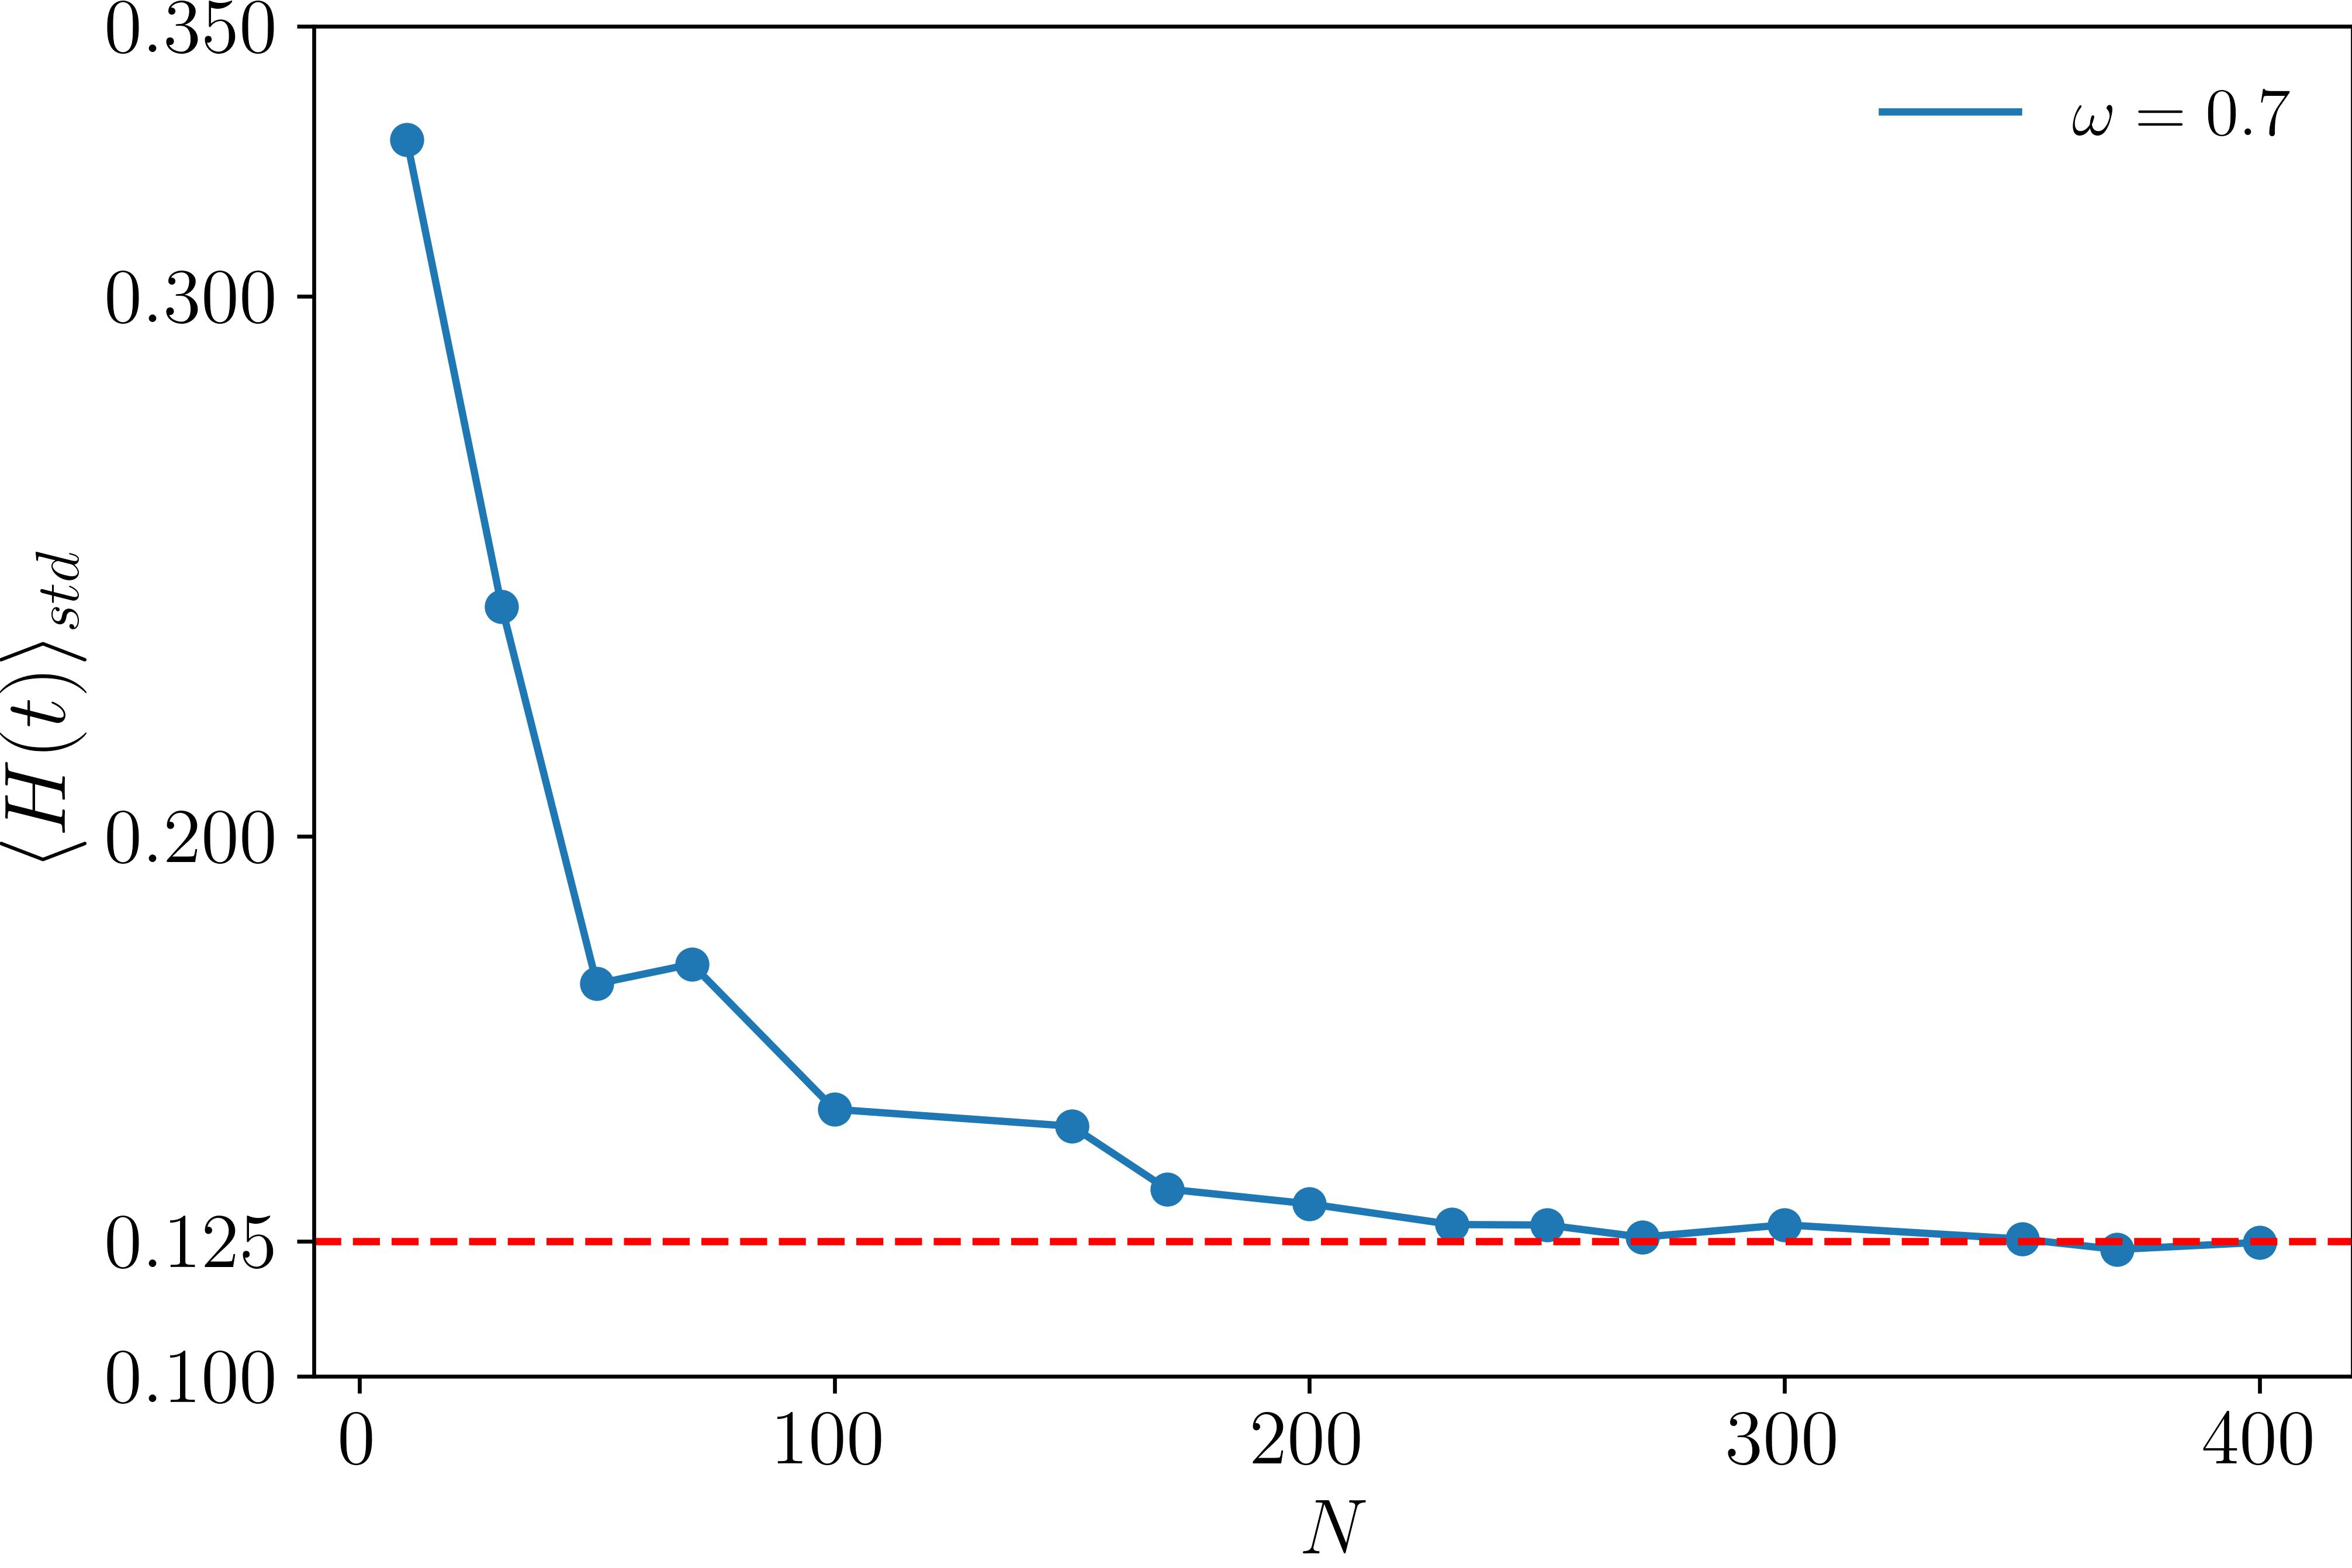
\includegraphics[width=7cm]{hbar_avg_std_w0.7.jpg}
	\caption{Variation of $\expval{H(t)}_{std}$ with system size(N) at small frequency $\omega=0.7$. $\expval{H(t)}_{std}$ is found to decrease as N increases and at thermodynamic limit it reaches 0.125.}
	\label{fig:std_N}
\end{textblock*}
}


\vskip 1.5cm
\item The referee says,``\textit{In the conclusion, it is useful to comment on whether this method could be adapted (related to my point 2) to other generic models (say
	XXZ models). }"\\

\response{

}
\vskip 1cm 
\noindent \textbf{Summary of important changes to the  manuscript}


\begin{enumerate}
\item 
\end{enumerate}

\bibliography{dmbl_refs}


\end{document}
